%%%%%%%%%%%%%%%%%%%%%%%%%%%%%%%%%%%%%%%%%%%%%%%%%%%%%%%%%%%%%%%%%%%%%%%%%%%%%%%%
% Archivo LaTeX para el informe final de la metaheurística RumorFlow (RF)
%
% Versión final con mejoras en el análisis y adición de conclusiones.
% REVISADO Y CORREGIDO POR EL PROFESOR
%%%%%%%%%%%%%%%%%%%%%%%%%%%%%%%%%%%%%%%%%%%%%%%%%%%%%%%%%%%%%%%%%%%%%%%%%%%%%%%%

\documentclass[11pt,a4paper]{article}

% --- PAQUETES ---
\usepackage[utf8]{inputenc}
\usepackage[T1]{fontenc}
\usepackage[spanish]{babel}
\usepackage{geometry}
\usepackage{graphicx}
\usepackage{booktabs}
\usepackage{tabularx}
\usepackage{amsmath}
\usepackage{amssymb}
\usepackage{algorithm}
\usepackage[noend]{algpseudocode} % Paquete para pseudocódigo
\usepackage{hyperref}
\usepackage{subcaption} % Para subfiguras

% --- CONFIGURACIÓN DE PAQUETES ---
\geometry{a4paper, margin=1in}
\hypersetup{
    colorlinks=true,
    linkcolor=blue,
    citecolor=green,
    urlcolor=cyan,
    pdftitle={RumorFlow (RF): Una Metaheurística de Inteligencia Colectiva},
    pdfauthor={Gabriel Sánchez Muñoz},
    bookmarks=true,
    pdfpagemode=FullScreen,
}
\renewcommand{\algorithmicrequire}{\textbf{Entrada:}}
\renewcommand{\algorithmicensure}{\textbf{Salida:}}

% --- INFORMACIÓN DEL DOCUMENTO ---
\title{\textbf{RumorFlow (RF): Una Metaheurística de Inteligencia Colectiva Inspirada en la Dinámica Social}}
\author{Gabriel Sánchez Muñoz}
\date{\today}

\begin{document}

\maketitle
\thispagestyle{empty}

\newpage
\tableofcontents
\newpage

\section{Introducción y Motivación}
La comunicación es un aspecto fundamental de las sociedades humanas. 
Desde hace milenios, la información, y con ella los mitos, leyendas y rumores, 
se ha transmitido de boca en boca, adaptándose y evolucionando con cada interacción. 
Este proceso dinámico de propagación y modificación de la información en una 
red social sirve como inspiración para una nueva metaheurística.

\vspace{0.5cm}

Este trabajo presenta \textbf{RumorFlow (RF)}, una metaheurística poblacional 
que modela la dinámica social de la propagación de un rumor. RF opera sobre una 
población de soluciones estructurada como un grafo de relaciones, donde los 
individuos (soluciones) se comunican entre sí, propagando y refinando sus 
``versiones del rumor'' (soluciones candidatas) a lo largo del tiempo. 
El objetivo es explorar cómo esta analogía social puede ser un paradigma 
eficaz para la optimización de problemas complejos.

\vspace{0.5cm}

La principal deficiencia que RF busca abordar en otros algoritmos poblacionales es 
su modelo de interacción, a menudo simplificado. En un Algoritmo Genético canónico, 
la selección para el cruce es global (panmixia), mientras que en PSO la influencia 
del "mejor global" crea una topología en estrella. RF propone un modelo más descentralizado 
y realista, donde la información (buenas características de una solución) fluye localmente 
a través de una topología de red que, además, puede evolucionar.

\vspace{0.5cm}

Además de una idea intuitiva sobre la propagación de los rumores, hay una sólida base
teórica ampliamente estudiada sobre estos aspectos. Desde la sociología y la epidemiología 
matemática, se han desarrollado modelos, como el canónico modelo SIR (Susceptible-Infectado-Recuperado), 
que tratan la difusión de información de forma análoga a la propagación de un virus. Estos modelos 
proporcionan un marco riguroso para entender cómo una idea nace, se expande a través de 
una red de contactos, se transforma y eventualmente se ``ahoga'' o pierde relevancia. 
Es precisamente esta base teórica la que motiva el diseño de RumorFlow, con el 
objetivo de traducir los principios fundamentales de la difusión social en una 
nueva y potente estrategia de optimización.

\section{El Algoritmo RumorFlow}

RumorFlow es una metaheurística poblacional que opera sobre un conjunto de $N$
soluciones $P = \{ s_1, s_2, \dots s_N \}$, donde cada solución $s_i$ representa un punto 
en el espacio de búsqueda. Una de las propuesta de RumotFlow es dotar a esta población de 
estructura de grafo $G = (V,E)$ orientado, donde los vértices $V$ son las soluciones $V_i = s_i$, y 
las aristas definen las vías de comunicación unidireccional permitidas entre ellas. La metáfora del rumor 
se traduce en los componentes del algoritmo como se describe en la Tabla ~\ref{tab:conceptos}.

\vspace{0.5cm}

\begin{table}[h!]
\centering
\caption{Correspondencia entre los conceptos del rumor y su implementación en RumorFlow.}
\label{tab:conceptos}
\small
\begin{tabularx}{\textwidth}{>{\raggedright\arraybackslash}p{3.5cm} >{\raggedright\arraybackslash}p{3cm} >{\raggedright\arraybackslash}p{5.5cm} >{\raggedright\arraybackslash}X}
\toprule
\textbf{Concepto del Rumor} & \textbf{Implementación} & \centering \textbf{Explicación} & \textbf{Explotación vs. Exploración} \\
\midrule
\textbf{Población/Sociedad} & \textbf{Grafo de solcuiones $G = (V,Ec)$} & En lugar de una lista de soluciones, la población es una red social. Cada solución es un ``individuo'' (nodo del grafo). & Depende de la topología del grafo. \\
\addlinespace
\textbf{Las conexiones sociales} & \textbf{Aristas del grafo} & Una arista $(s_i,s_j) \in E$ significa que la solución $s_i$ puede ``contarle un rumor'' a $s_j$ & \\
\addlinespace
\textbf{La versión del rumor} & \textbf{Cromosoma (Solución)} & Cada individuo tiene su propia versión del rumor, que no es más que una solución candidata al problema. & \\
\addlinespace
\textbf{Contar el rumor} & \textbf{Operador de propagación} & Un individuo propagador $(s_i)$ transmite su rumor a un vecino $(s_j)$. El nuevo estado de $s_j$ se genera combinando ambos, de manera sesgada hacia el mejor rumor. & Depende de la profundidad de propagación. \\
\addlinespace
\textbf{Malentendidos/olvidos} & \textbf{Operador de mutación} & Se simula el ``teléfono roto'' o el olvido de detalles cambiando al azar partes de una solución. & Exploración \\
\addlinespace
\textbf{Cambios en la red social} & \textbf{Mutación del grafo} & Se cambian las aristas del grafo elmininado y añadiendo conexiones para que las ideas no se estanquen en los mismos grupos. & Exploración \\
\bottomrule
\end{tabularx}
\end{table}

\vspace{0.5cm}

La principal novedad de \textbf{RumorFlow} frente a otros algoritmos es su 
\textbf{estructura de grafo explícita y dinámica} y su \textbf{operador de propagación asimétrico}. 
Mientras que en otros algoritmos las interacciones suelen ser aleatorias o 
globales, en RF solo los individuos conectados pueden interactuar. Además, 
el operador de cruce (la propagación del rumor) está diseñado para ser 
``inteligente'', favoreciendo la influencia de las mejores soluciones 
de una manera más análoga a la dinámica social, y el propio grafo evoluciona, 
adaptando las rutas de comunicación.

\subsection{Topologías de la Población}

Dependiendo de la estructura del grafo de población,
la propagación tendrá diferentes comportamientos, a veces favoreciendo una explotación muy 
agresiva y otras veces conservando la diversidad, con el coste de ralentizar la velocidad de 
la optimización.

Con el fin de estudiar el comportamiento del algoritmo bajo diferentes topologías, se han 
diseñado los siguientes tipos de grafos de población:

\begin{itemize}
    \item \textbf{Completo:} En este caso, la población se comportará como la de un algoritmo genético tradicional.
    Todos se pueden comunicar con todos, lo que provoca que la propagación sea demasiado explosiva. Aunque ajustando 
    el operador podría ser una población viable, la estructura de grafo completo no cuadra con la filosofía detrás 
    del algoritmo.
    \item \textbf{Ciclo:} El caso opuesto al grafo completo. Cada solución solo está conectada con otras dos, formando 
    un ciclo. Esta estructura limita en exceso las conexiones de cada individuo, por lo que no es capaz de explorar 
    más allá de un vecindario reducido. 
    \item \textbf{Aleatorio:} La estructura más prometedora y que representa de manera simplificada una red social.
    Ajustando adecuadamente la densidad de aristas, se consigue que el operador de propagación expanda las buenas 
    soluciones, pero también se mantiene la diversidad al tener cada individuo un mayor número de vecinos con los que intercambiar rumores.
    \item \textbf{Grupos aleatorios:} Tratando de buscar más similitudes con el comportamiento social real, esta 
    estructura genera grupos de manera aleatoria, con mayor densidad de comunicación dentro de cada grupo y menor entre grupos.
    \item \textbf{Grupos no aleatorios:} Se explora la idea de dar un orden a la estructura de grupos aleatorios para 
    tener más control sobre la topología.
\end{itemize}

Para el desarrollo del algoritmo se utiliza una población aleatoria con una densidad de aristas variable entre 0.05 y 0.25, es decir, 
entre 5 y 25 vecinos por nodo en promedio. Esta estructura es la que mejores resultados ha brindado, aunque no se descarta que otro tipo 
de poblaciones, configuradas de distinta manera, puedan mejorar el comportamiento del algoritmo.

\subsection{Funcionamiento del Algoritmo}

El flujo principal de RumorFlow se describe en el Algoritmo~\ref{alg:rf}. 
El proceso comienza inicializando una población de forma aleatoria y su grafo de relaciones. 
En cada ciclo, se seleccionan los individuos más prometedores (``propagadores'') 
mediante un torneo, que propagan sus soluciones a sus vecinos a través de la red.
Además, se muta un cierto porcentaje de las soluciones, y cada ciertas generaciones 
se muta la red social (el grafo) para cambiar las conexiones.

\subsection{El Operador de Propagación}
El núcleo de RF es el operador `PropagarRumor` (Algoritmo~\ref{alg:propagate}). 
A diferencia de un cruce convencional, la propagación es un proceso iterativo en rondas. 
Los individuos ``convencidos'' en una ronda se convierten en propagadores en la siguiente, 
creando un efecto dominó que permite a las buenas soluciones extenderse rápidamente por la red. 
El cruce (`CruceInteligente`) es asimétrico: la nueva solución se genera en un rango 
sesgado hacia la mejor solución entre la del receptor y la del propagador.

\newpage

\section{Diseño Experimental y Resultados}
Para ejecutar el algoritmo, fue necesario probar y elegir diferentes parámetros.
Los parámetros utilizados en todos los experimentos se detallan en la Tabla~\ref{tab:parametros}.

\begin{table}[h!]
\centering
\caption{Parámetros de configuración para todos los experimentos de RumorFlow.}
\label{tab:parametros}
\begin{tabularx}{\textwidth}{l l >{\raggedright\arraybackslash}X}
\toprule
\textbf{Parámetro} & \textbf{Valor} & \textbf{Descripción} \\
\midrule
\texttt{mutation\_prob} & 0.1 & Porcentaje de individuos mutados por generación \\
\texttt{mutation\_intensity} & 0.1 & Porcentaje de genes mutados de un individuo \\
\texttt{population\_size} & 100 & Número de individuos de la población \\
\texttt{max\_rounds} & 2 & Número máximo de rondas para la propagación \\
\texttt{select\_percentage} & 0.2 & Porcentaje de “propagadores” en una generación \\
\texttt{tournament\_ratio} & 0.2 & Porcentaje de la población que disputa el torneo de selección \\
\bottomrule
\end{tabularx}
\end{table}

Esta selección ha dado buenos resultados, pero una investigación más profunda sobre posibles valores alternativos o 
la optimización de parámetros por diferentes métodos podrían sugerir mejores elecciones.


Los algoritmos fueron ejecutados sobre un conjunto estándar de funciones de benchmark (CEC) con dimensiones D=10, 30 y 50 para evaluar su escalabilidad. Los resultados se presentan como el ranking promedio del algoritmo en diferentes puntos del consumo de evaluaciones.

\subsection{Algoritmos de Comparación}
Para evaluar la competitividad de RumorFlow, es crucial situarlo en el 
contexto de otras metaheurísticas establecidas, especialmente aquellas 
con las que se compara directamente en este estudio.

\begin{itemize}
    \item \textbf{Particle Swarm Optimization (PSO):} Es una de las metaheurísticas 
    de inteligencia colectiva más conocidas. Se inspira en el comportamiento de las 
    bandadas de pájaros. Cada solución, o ``partícula'', ajusta su trayectoria en el 
    espacio de búsqueda basándose en su propia mejor experiencia histórica (\textit{personal best}) 
    y en la mejor experiencia del conjunto de la población (\textit{global best}). 
    A diferencia de RF, la topología de comunicación en el PSO canónico es global 
    (estrella) y no utiliza un operador de cruce explícito entre soluciones.
    
    \item \textbf{Differential Evolution (DE):} Es un algoritmo evolutivo potente y 
    ampliamente utilizado, especialmente para problemas de optimización de valor real. 
    Su principal característica es el operador de mutación, que crea nuevos vectores de 
    solución combinando la diferencia vectorial de otros individuos de la población. 
    Aunque es poblacional, DE no estructura la población en un grafo explícito que 
    restrinja las interacciones como lo hace RF.
    
    \item \textbf{Artificial Ecosystem-based Optimization (AEO):} Es una metaheurística 
    más reciente inspirada en el flujo de energía en un ecosistema. Modela tres 
    comportamientos principales: producción, consumo y descomposición. Cada rol 
    corresponde a diferentes estrategias de exploración y explotación. AEO gestiona la 
    población de forma global, mientras que RF se basa en interacciones locales definidas por un grafo.
\end{itemize}

\subsection{Análisis de Rendimiento del Algoritmo Base (RF)}

En primer lugar, se ha ejecutado el algoritmo base, tal y como se detalla 
en su pseudocódigo (Algoritmo \ref{alg:rf}).

\begin{table}[h!]
\centering \caption{Ranking promedio para RF base, D=10.} \label{tab:rf_d10}
\begin{tabular}{lrrrrrr} 
    \toprule Algoritmo & 1\% & 10\% & 25\% & 50\% & 75\% & 100\% \\ 
    \midrule AEO & 1.817 & 2.517 & 2.850 & 3.150 & 3.150 & 3.150 \\ 
    DE  & 3.867 & 2.200 & 1.858 & 1.783 & 1.850 & 1.850 \\ 
    PSO & 3.083 & 3.450 & 3.250 & 2.983 & 2.833 & 2.783 \\ 
    RF  & 1.233 & 1.833 & 2.042 & 2.083 & 2.150 & 2.217 \\ 
    \bottomrule \end{tabular} \end{table}
\begin{table}[h!]
\centering \caption{Ranking promedio para RF base, D=30.} \label{tab:rf_d30}
\begin{tabular}{lrrrrrr} 
    \toprule Algoritmo & 1\% & 10\% & 25\% & 50\% & 75\% & 100\% \\ 
    \midrule AEO & 1.917 & 3.083 & 3.283 & 3.383 & 3.383 & 3.383 \\ 
    DE  & 3.833 & 2.133 & 1.800 & 1.600 & 1.533 & 1.500 \\ 
    PSO & 3.083 & 3.483 & 3.450 & 3.317 & 3.267 & 3.183 \\ 
    RF  & 1.167 & 1.300 & 1.483 & 1.700 & 1.817 & 1.933 \\ 
    \bottomrule \end{tabular} \end{table}
\begin{table}[h!]
\centering \caption{Ranking promedio para RF base, D=50.} \label{tab:rf_d50}
\begin{tabular}{lrrrrrr} 
    \toprule Algoritmo & 1\% & 10\% & 25\% & 50\% & 75\% & 100\% \\ 
    \midrule AEO & 2.083 & 3.183 & 3.350 & 3.350 & 3.383 & 3.350 \\ 
    DE  & 3.833 & 2.167 & 1.900 & 1.800 & 1.767 & 1.667 \\ 
    PSO & 2.983 & 3.450 & 3.383 & 3.383 & 3.350 & 3.383 \\ 
    RF  & 1.100 & 1.200 & 1.367 & 1.467 & 1.500 & 1.600 \\ 
    \bottomrule \end{tabular} \end{table}

Las Tablas \ref{tab:rf_d10} a \ref{tab:rf_d50} revelan un patrón de comportamiento inequívoco para el algoritmo RF base. En las fases iniciales de la búsqueda (1-10\% de las evaluaciones), RF es extraordinariamente dominante, superando a todas las metaheurísticas de comparación. Este rendimiento valida la potencia de su operador de propagación, que disemina eficientemente las características de las soluciones prometedoras a través de la red social. Sin embargo, este mismo mecanismo es su talón de Aquiles. A medida que avanza la ejecución, el rendimiento de RF decae drásticamente, siendo superado por algoritmos como DE. Este comportamiento es un síntoma clásico de \textbf{convergencia prematura}. El algoritmo exhibe una explotación tan agresiva que la diversidad de la población se colapsa rápidamente, como se ilustra conceptualmente en la Figura~\ref{fig:dist_rf}. Una vez estancado en un óptimo local, carece de los mecanismos de exploración necesarios para escapar y continuar la búsqueda global. El diagnóstico es claro: RF posee un motor de explotación de alto potencial, pero está desequilibrado por una estrategia de exploración insuficiente.
\begin{figure}[h!]
    \centering
    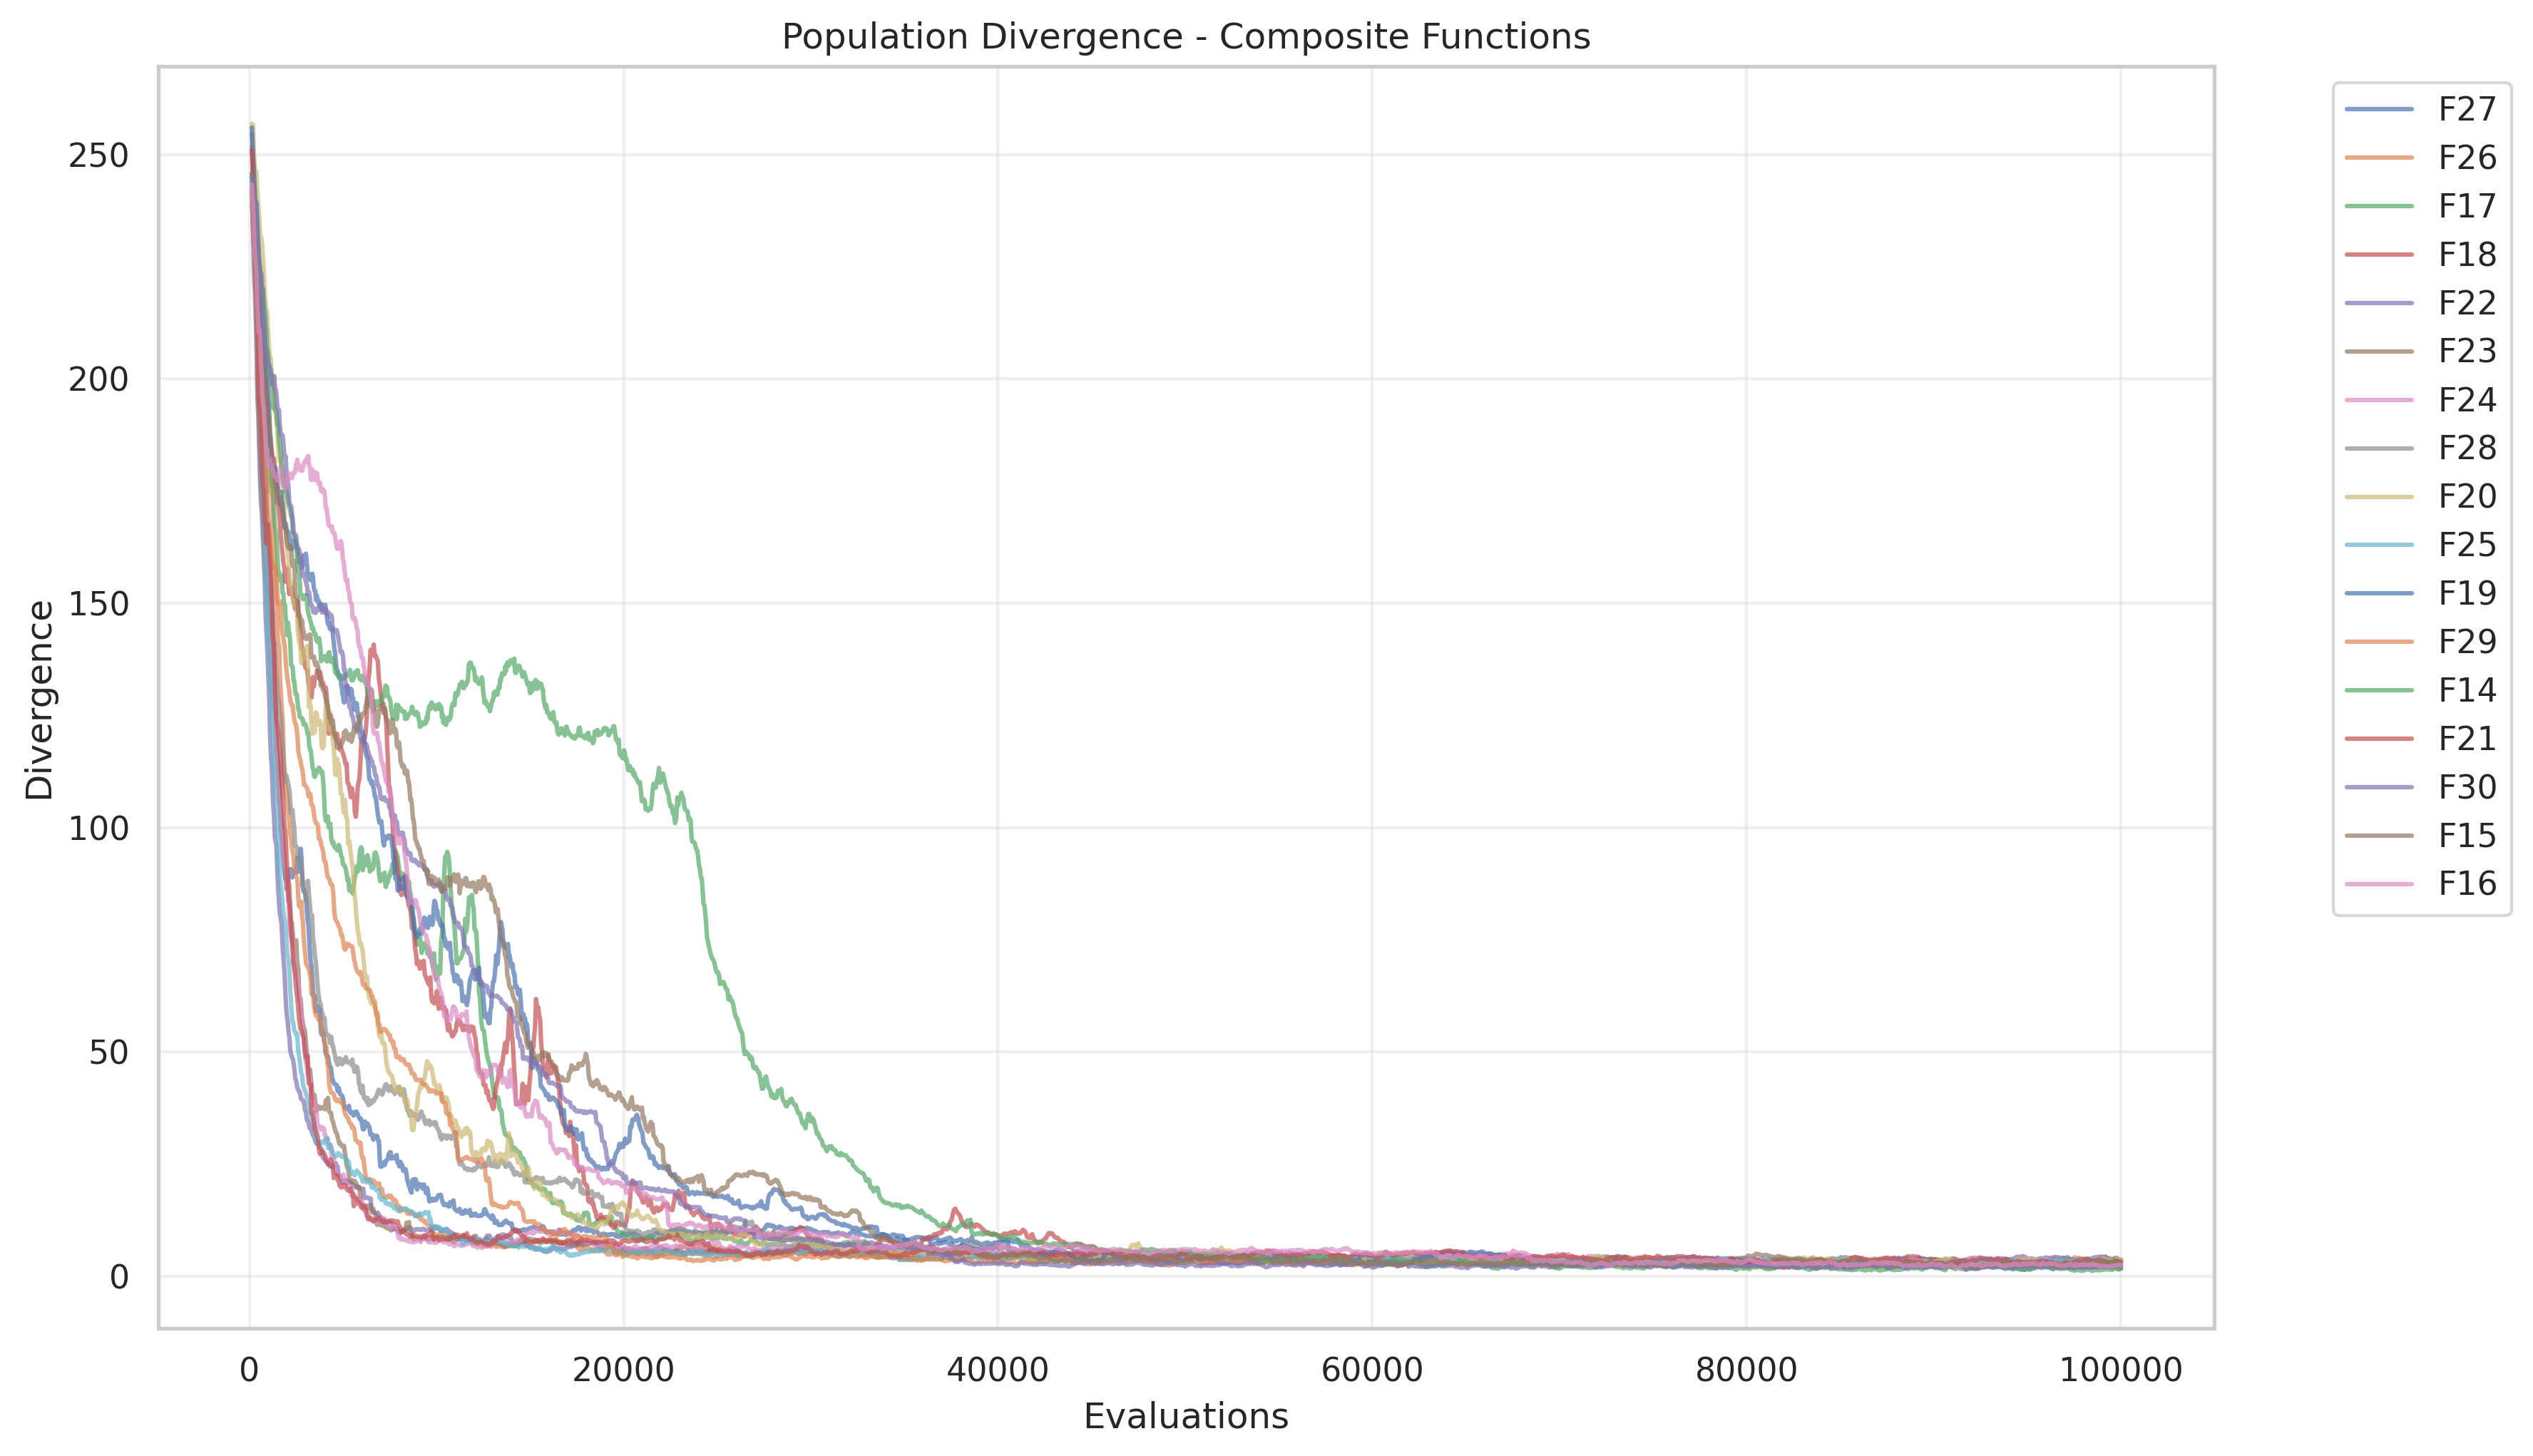
\includegraphics[width=0.8\textwidth]{assets/composite_divergence.png}
    \caption{Se ve claramente que para la mayoría de funciones a optimizar, la diversidad cae rápidamente.}
    \label{fig:dist_rf}
\end{figure}

\subsection{Hibridación con Búsqueda Local (RF-BL)}
La primera hipótesis de mejora es que, si se aplica una búsqueda local a 
las soluciones prometedoras generadas por RF, se podría intensificar la 
explotación y alcanzar mejores óptimos. Es decir, si podemos trabajar con mejores soluciones 
cuanto antes, esto puede guiar la población hacia óptimos de mayor calidad.

\begin{table}[h!]
\centering \caption{Ranking promedio de RF-BL para D=10.} \label{tab:rfbl_d10}
\begin{tabular}{lrrrrrr} 
    \toprule Algoritmo & 1\% & 10\% & 25\% & 50\% & 75\% & 100\% \\ 
    \midrule AEO   & 1.683 & 2.483 & 2.783 & 3.083 & 3.067 & 3.083 \\ 
    DE    & 3.867 & 2.133 & 1.833 & 1.783 & 1.850 & 1.850 \\ 
    PSO   & 3.083 & 3.417 & 3.267 & 2.883 & 2.783 & 2.750 \\ 
    RF-BL & 1.367 & 1.967 & 2.117 & 2.250 & 2.300 & 2.317 \\ 
    \bottomrule \end{tabular} \end{table}
\begin{table}[h!]
\centering \caption{Ranking promedio de RF-BL para D=30.} \label{tab:rfbl_d30}
\begin{tabular}{lrrrrrr} 
    \toprule Algoritmo & 1\% & 10\% & 25\% & 50\% & 75\% & 100\% \\ 
    \midrule AEO   & 1.883 & 3.117 & 3.317 & 3.417 & 3.417 & 3.417 \\ 
    DE    & 3.833 & 2.133 & 1.767 & 1.633 & 1.533 & 1.467 \\ 
    PSO   & 3.083 & 3.483 & 3.433 & 3.383 & 3.317 & 3.250 \\ 
    RF-BL & 1.200 & 1.267 & 1.483 & 1.567 & 1.733 & 1.867 \\ 
    \bottomrule \end{tabular} \end{table}
\begin{table}[h!]
\centering \caption{Ranking promedio de RF-BL para D=50.} \label{tab:rfbl_d50}
\begin{tabular}{lrrrrrr} 
    \toprule Algoritmo & 1\% & 10\% & 25\% & 50\% & 75\% & 100\% \\ 
    \midrule AEO   & 2.083 & 3.183 & 3.350 & 3.350 & 3.383 & 3.350 \\ 
    DE    & 3.833 & 2.167 & 1.967 & 1.867 & 1.833 & 1.733 \\ 
    PSO   & 2.983 & 3.450 & 3.383 & 3.350 & 3.350 & 3.383 \\ 
    RF-BL & 1.100 & 1.200 & 1.300 & 1.433 & 1.433 & 1.533 \\ 
    \bottomrule \end{tabular} \end{table}

Los resultados de la hibridación con búsqueda local (Tablas \ref{tab:rfbl_d10}-\ref{tab:rfbl_d50}) son un \textbf{hallazgo diagnóstico crucial}. A pesar de la hipótesis de que una mayor intensificación podría mejorar la calidad de la convergencia, los datos muestran que RF-BL no ofrece una mejora sustancial sobre el algoritmo base. El perfil de rendimiento —un inicio fuerte seguido de un estancamiento— permanece inalterado. Este resultado negativo refuta la hipótesis inicial y nos permite concluir con firmeza que el cuello de botella de RF no es una falta de poder de explotación. De hecho, el algoritmo ya es tan eficiente en la intensificación que añadir una búsqueda local es redundante. El problema fundamental y no resuelto es la \textbf{pérdida catastrófica de diversidad}. Este experimento, aunque no produjo un algoritmo superior, fue fundamental para reorientar correctamente la investigación hacia la gestión de la exploración.

\subsection{Mejora con Reinicialización (RF-R)}
Basado en la conclusión anterior, se diseña una nueva versión, 
RF-R, que incorpora un mecanismo de reinicialización. 

La reinicialización consiste en regenerar la población cuando 
la diversidad, medida como la distancia promedio entre las soluciones,
cae por debajo de un umbral predefinido. En particular, la población se regenera 
en el entorno de un centro aleatorio con un radio reducido. De esta manera, conseguimos 
alejarnos de óptimos locales y forzar la exploración en nuevas zonas del espacio de búsqueda.

Además, se preserva la mejor solución encontrada hasta el momento (elitismo) para no perder el progreso entre reinicializaciones.

El pseudocódigo de la reinicialización (Algoritmo \ref{alg:restart}) se encuentra en el Apéndice A.

\begin{table}[h!]
\centering \caption{Ranking promedio de RF-R para D=10.} \label{tab:rfr_d10}
\begin{tabular}{lrrrrrr} 
    \toprule Algoritmo & 1\% & 10\% & 25\% & 50\% & 75\% & 100\% \\ 
    \midrule AEO  & 1.483 & 2.550 & 2.883 & 3.183 & 3.250 & 3.317 \\ 
    DE   & 3.833 & 2.166 & 1.825 & 1.883 & 1.983 & 1.950 \\ 
    PSO  & 3.050 & 3.450 & 3.283 & 3.083 & 2.983 & 2.983 \\ 
    RF-R & 1.633 & 1.833 & 2.008 & 1.850 & 1.767 & 1.750 \\ 
    \bottomrule \end{tabular} \end{table}
\begin{table}[h!]
\centering \caption{Ranking promedio de RF-R para D=30.} \label{tab:rfr_d30}
\begin{tabular}{lrrrrrr} 
    \toprule Algoritmo & 1\% & 10\% & 25\% & 50\% & 75\% & 100\% \\ 
    \midrule AEO  & 1.917 & 3.050 & 3.283 & 3.417 & 3.417 & 3.417 \\ 
    DE   & 3.833 & 2.133 & 1.883 & 1.833 & 1.767 & 1.667 \\ 
    PSO  & 3.083 & 3.483 & 3.433 & 3.383 & 3.350 & 3.283 \\ 
    RF-R & 1.167 & 1.333 & 1.400 & 1.367 & 1.467 & 1.633 \\ 
    \bottomrule \end{tabular} \end{table}
\begin{table}[h!]
\centering \caption{Ranking promedio de RF-R para D=50.} \label{tab:rfr_d50}
\begin{tabular}{lrrrrrr} 
    \toprule Algoritmo & 1\% & 10\% & 25\% & 50\% & 75\% & 100\% \\ 
    \midrule AEO  & 2.083 & 3.183 & 3.350 & 3.350 & 3.383 & 3.350 \\ 
    DE   & 3.833 & 2.267 & 2.033 & 1.967 & 1.867 & 1.767 \\ 
    PSO  & 2.983 & 3.450 & 3.383 & 3.383 & 3.350 & 3.383 \\ 
    RF-R & 1.100 & 1.100 & 1.233 & 1.300 & 1.400 & 1.500 \\ 
    \bottomrule \end{tabular} \end{table}

La incorporación del mecanismo de reinicialización en RF-R valida de forma contundente la nueva hipótesis. Como se observa en las Tablas \ref{tab:rfr_d10}-\ref{tab:rfr_d50}, el rendimiento del algoritmo se transforma. RF-R no solo mantiene su competitividad inicial, sino que la sostiene a lo largo de toda la ejecución, llegando a superar a algoritmos robustos como DE en las fases finales, especialmente en dimensiones altas (D=30 y D=50). Este éxito se debe directamente a la gestión activa de la diversidad. Como se visualiza en las gráficas de la Figura \ref{fig:individual_div}, la reinicialización introduce picos periódicos en la diversidad poblacional, representando una inyección de nuevo material genético que permite al algoritmo escapar de la convergencia prematura. Cada reinicio actúa como un catalizador que permite a RF volver a desplegar su potente motor de explotación en una región diferente y prometedora del espacio de búsqueda, logrando un balance exploración-explotación mucho más eficaz.c
\begin{figure}[h!]
    \centering
    \begin{subfigure}[b]{0.45\textwidth}
        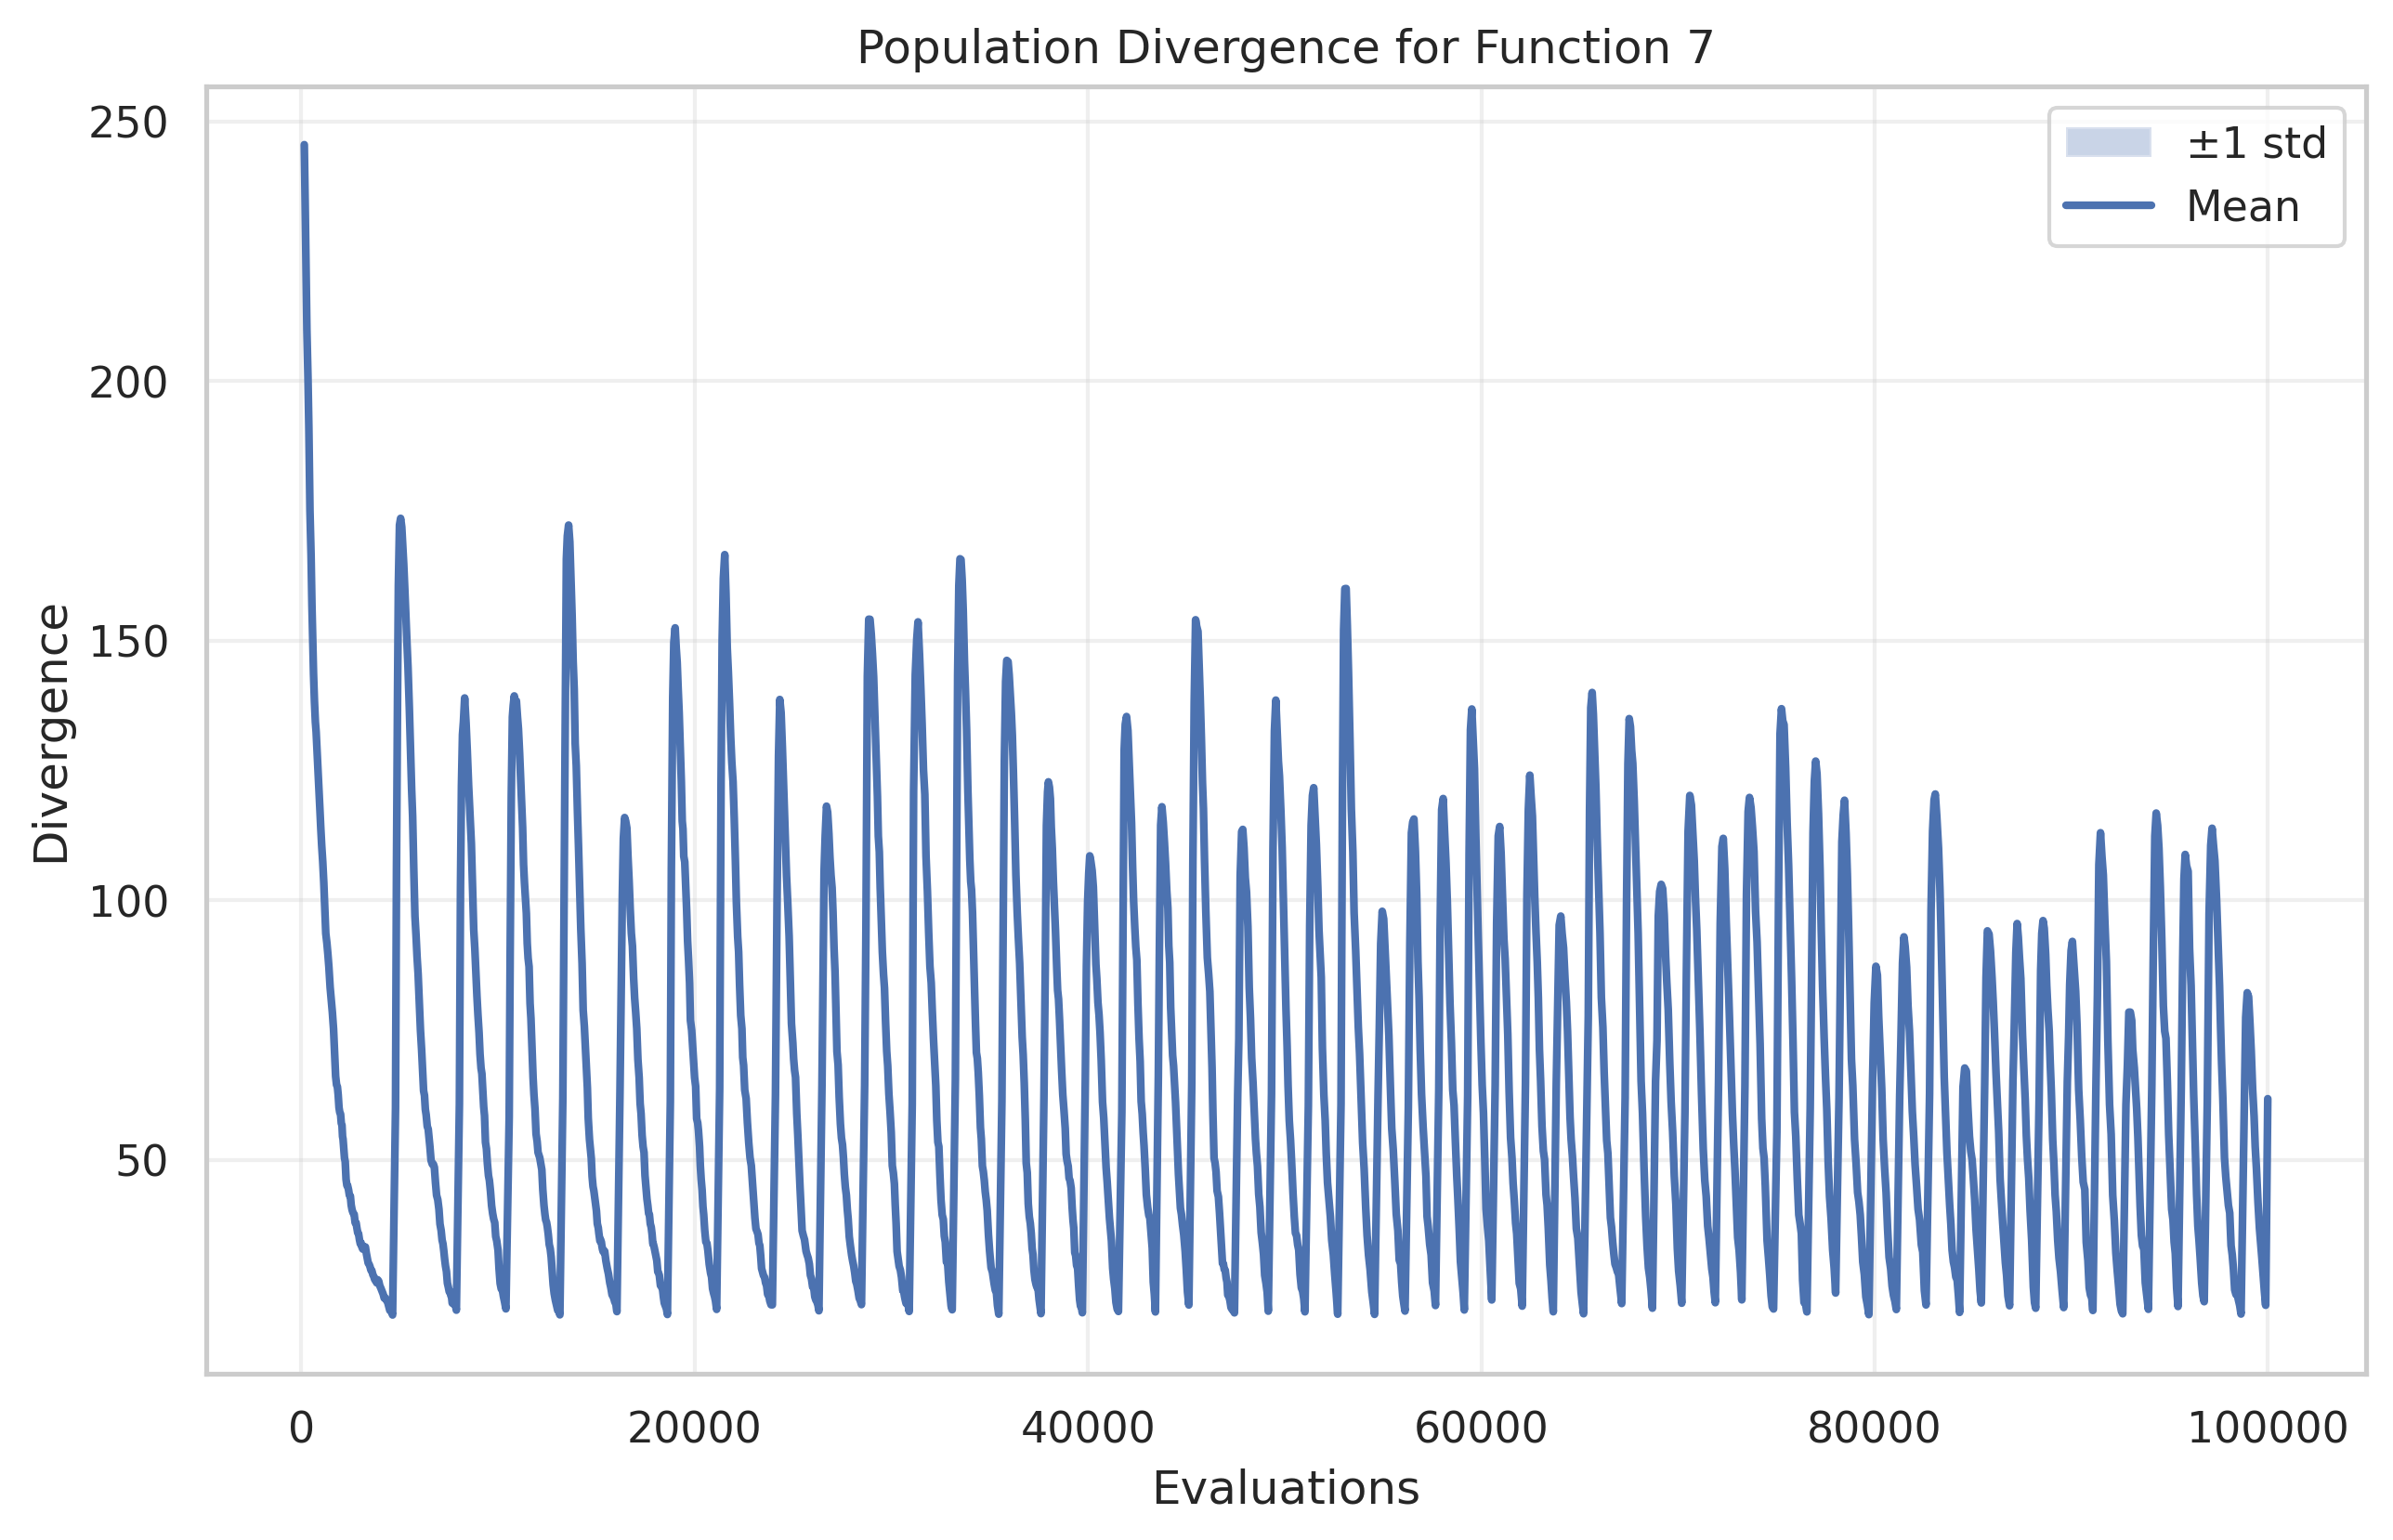
\includegraphics[width=\textwidth]{assets/F7_divergence.png}
        \caption{Función F7}
        \label{fig:f7_div}
    \end{subfigure}
    \hfill
    \begin{subfigure}[b]{0.45\textwidth}
        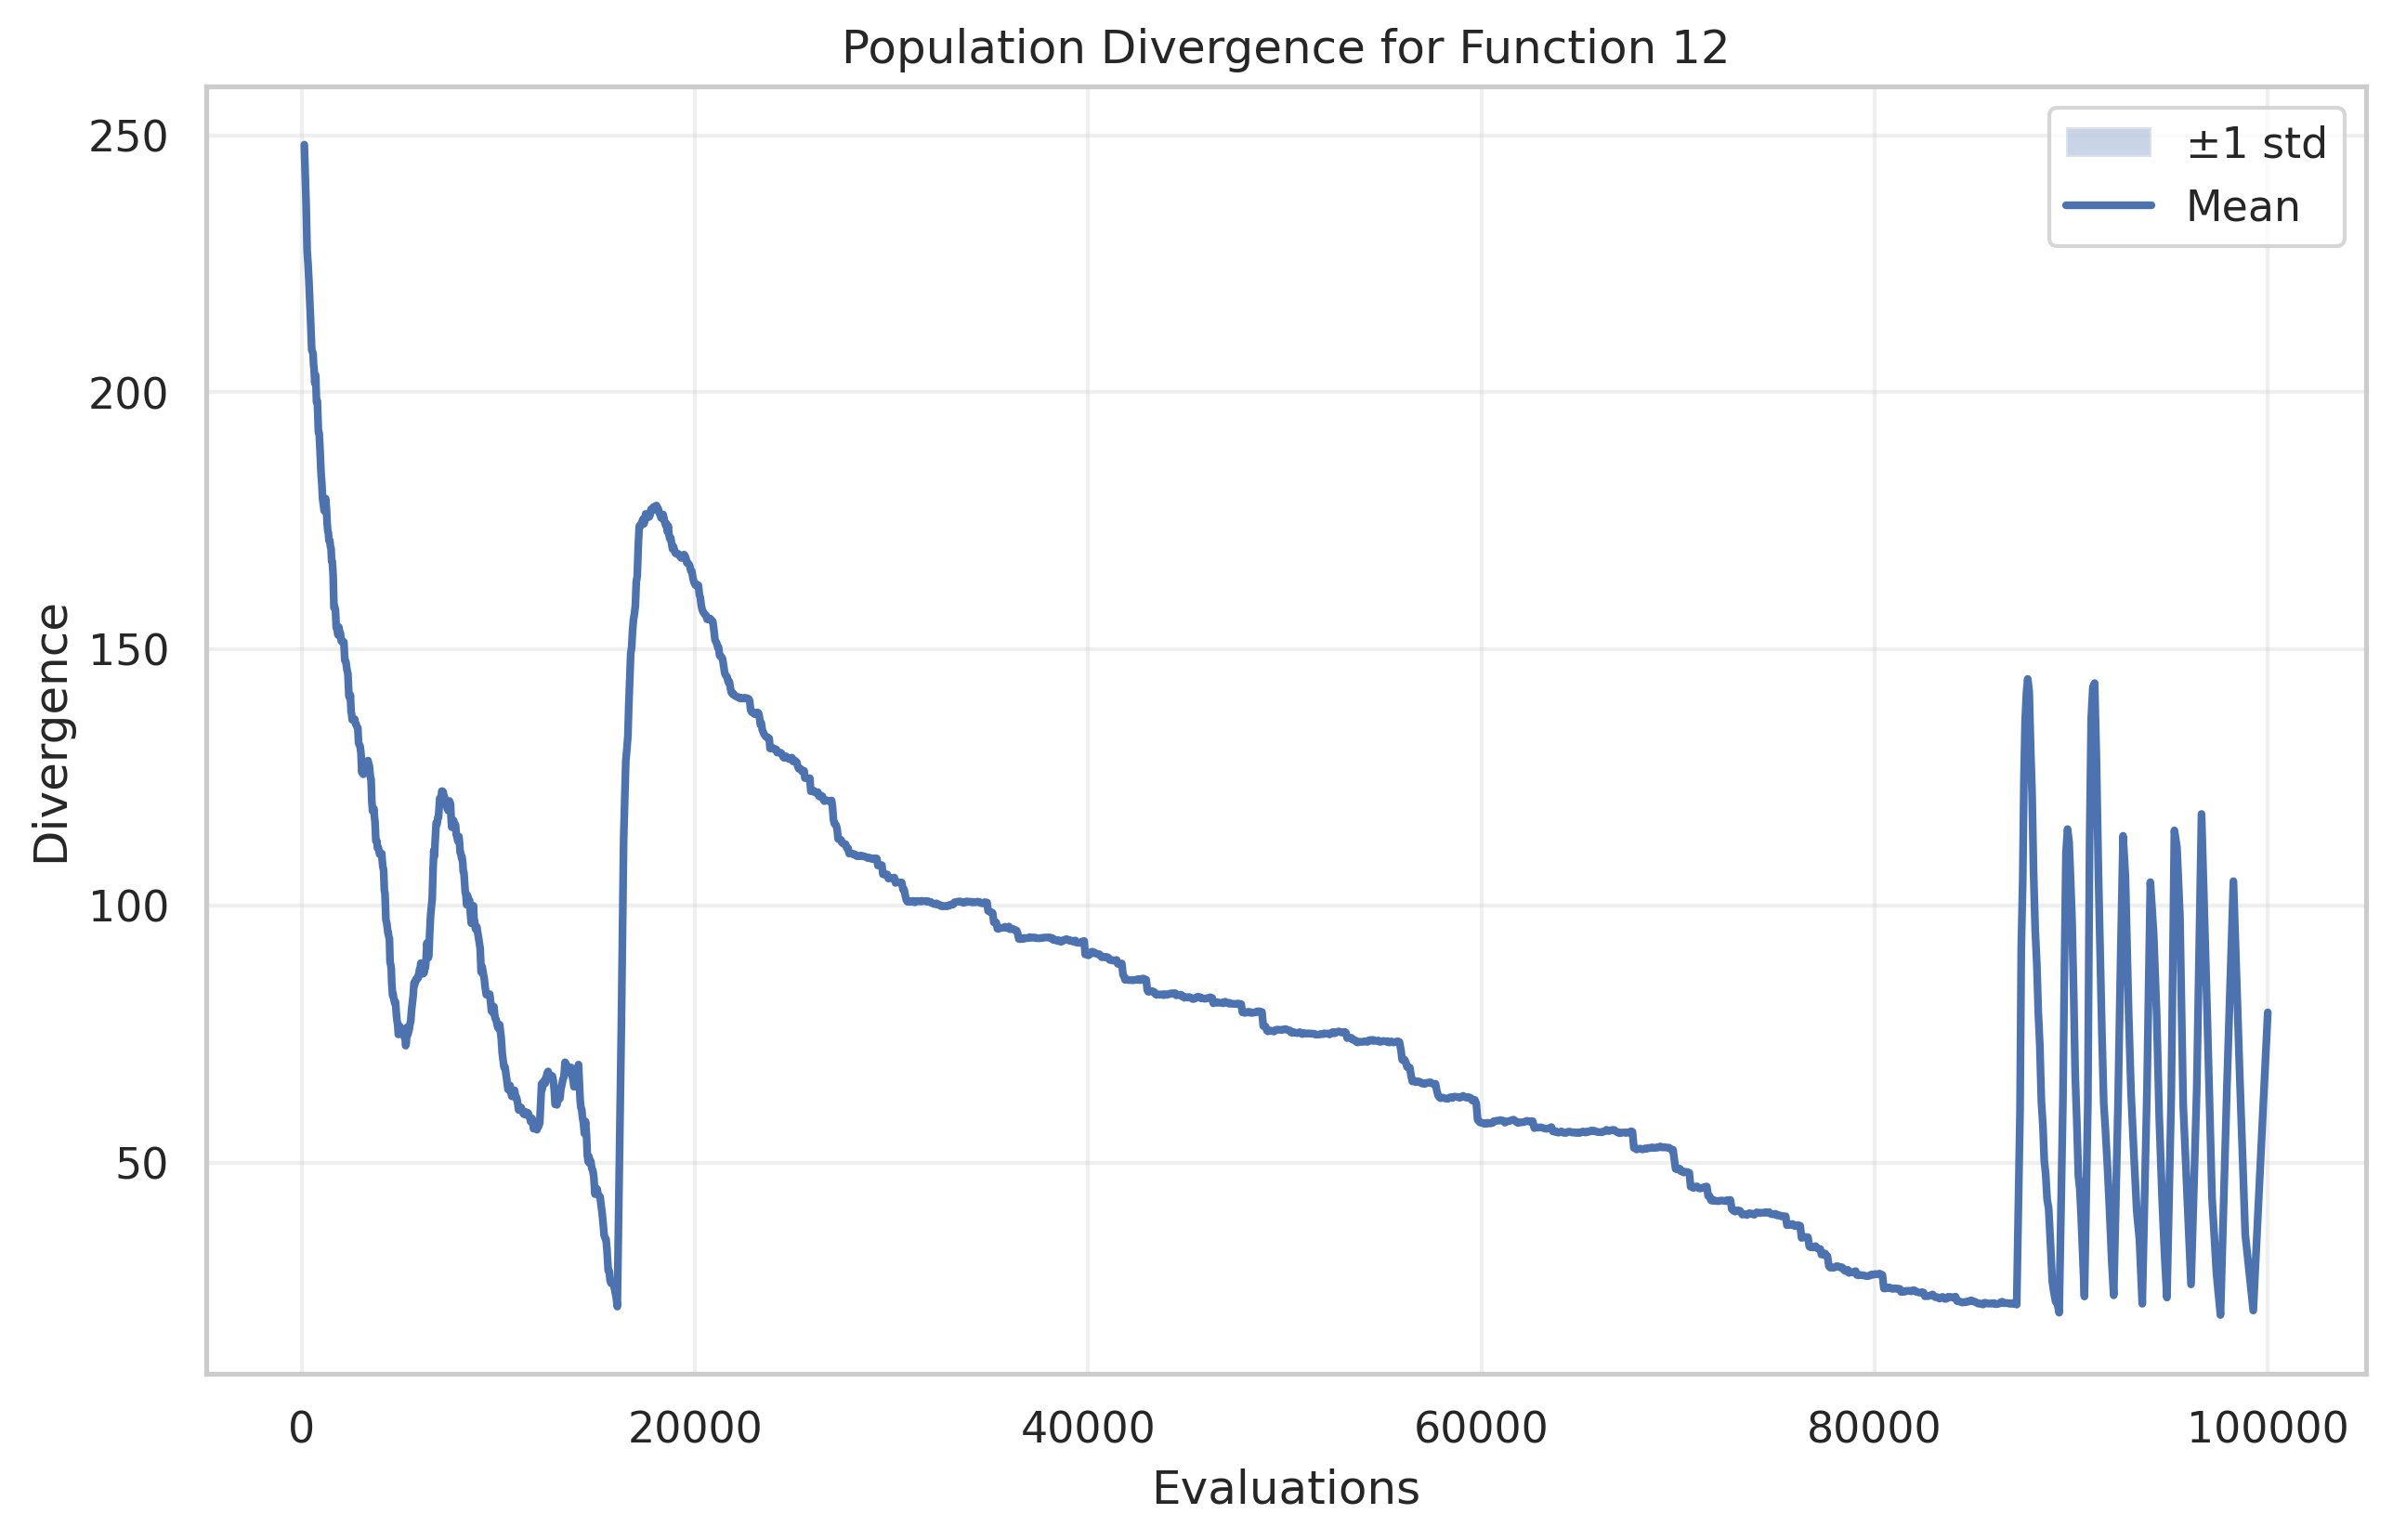
\includegraphics[width=\textwidth]{assets/F12_divergence.png}
        \caption{Función F12}
        \label{fig:f12_div}
    \end{subfigure}
    \hfill
    \begin{subfigure}[b]{0.45\textwidth}
        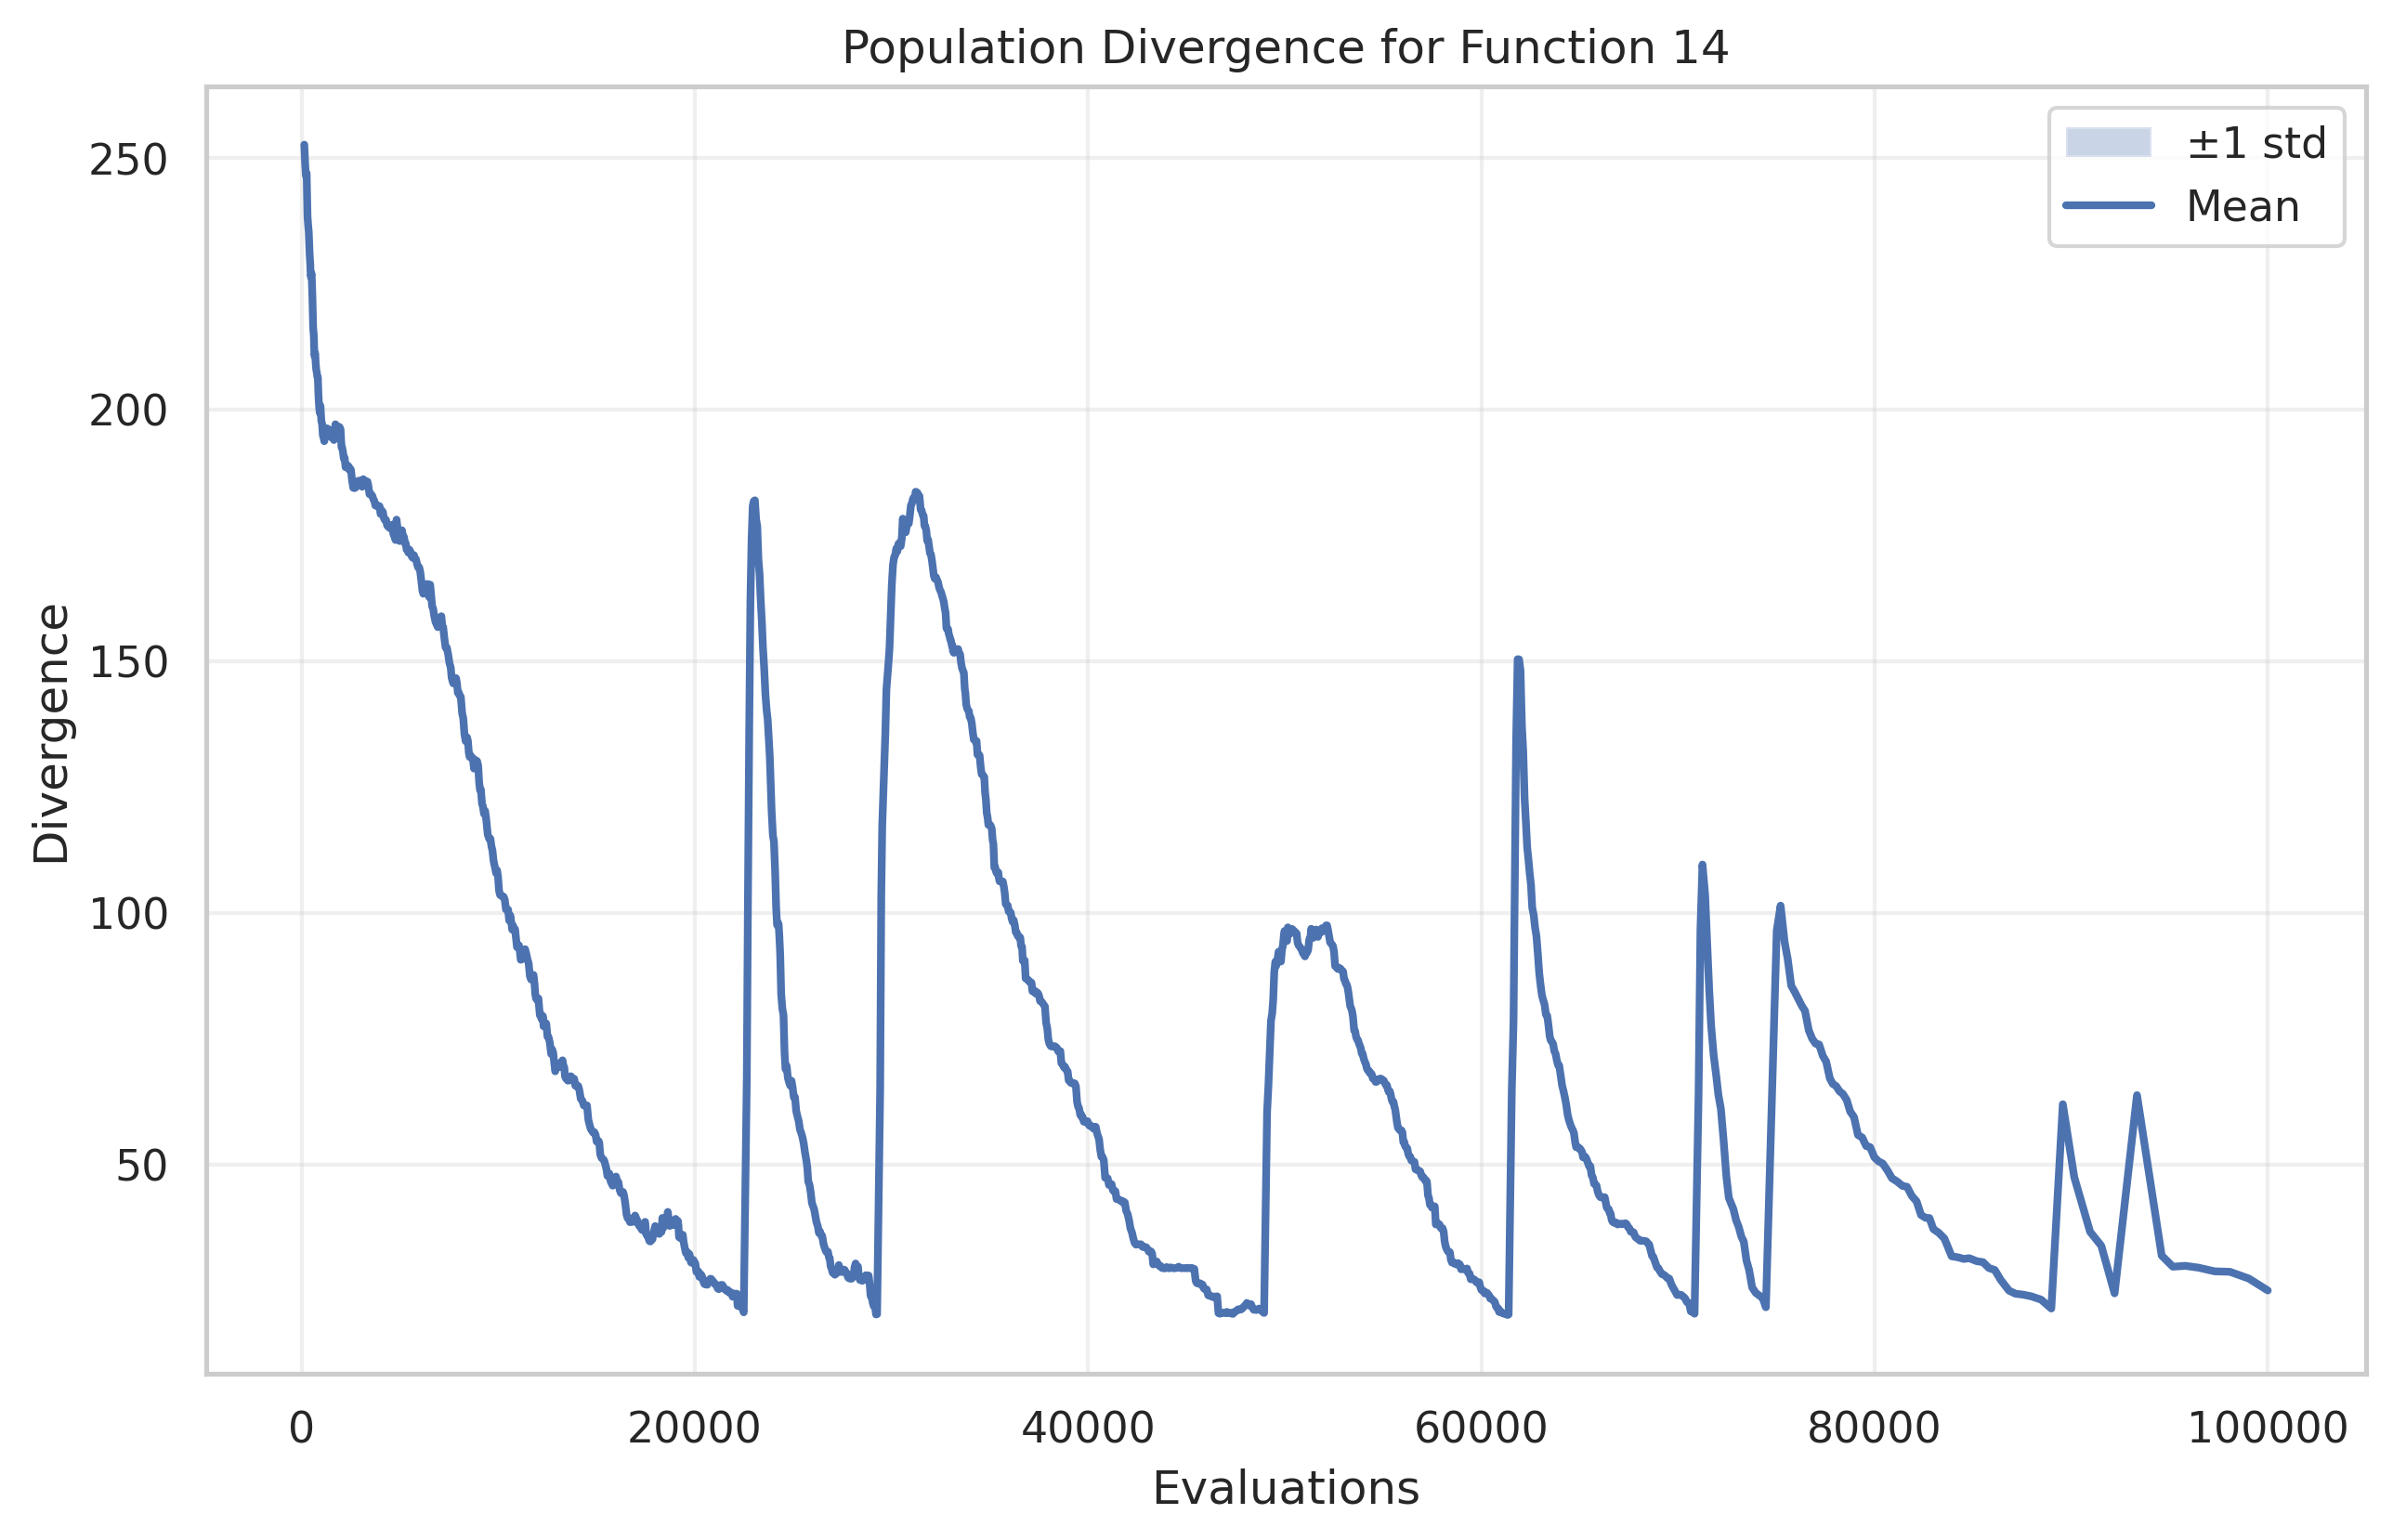
\includegraphics[width=\textwidth]{assets/F14_divergence.png}
        \caption{Función F14}
        \label{fig:f14_div}
    \end{subfigure}
    \caption{Análisis de la evolución de la diversidad en diferentes funciones de prueba. Se puede observar un patrón consistente en la pérdida temprana de diversidad en RF y la restauración periódica en RF-R.}
    \label{fig:individual_div}
\end{figure}

\subsection{Extensión Multi-Poblacional: GroupsRumorFlow (GRF)}
Observando el éxito de la reinicialización, se explora una mejora 
adicional. Una limitación de RF-R es que descarta a casi toda la 
población al reinicializar. Para solventarlo, se propone 
\textbf{GroupsRumorFlow (GRF)}, una arquitectura de dos fases:
\begin{enumerate}
    \item \textbf{Fase de Exploración Paralela:} Múltiples poblaciones 
    (grupos) ejecutan RF de forma independiente, explorando diferentes 
    zonas del espacio de búsqueda.
    \item \textbf{Fase de Explotación Conjunta:} Se recolectan los 
    mejores individuos de cada grupo para formar una nueva población 
    de élite, que es optimizada intensivamente con RF.
\end{enumerate}

Este enfoque busca combinar una amplia exploración global con una potente explotación final.

\begin{table}[h!]
\centering \caption{Ranking promedio de GRF para D=10.} \label{tab:grf_d10}
\begin{tabular}{lrrrrrr} \toprule Algoritmo & 1\% & 10\% & 25\% & 50\% & 75\% & 100\% \\ \midrule 
AEO & 1.017 & 2.583 & 2.950 & 3.217 & 3.367 & 3.383 \\
DE  & 3.733 & 2.033 & 1.833 & 1.833 & 2.083 & 2.083 \\
PSO & 2.417 & 3.517 & 3.350 & 3.083 & 3.050 & 3.050 \\
GRF & 2.833 & 1.867 & 1.867 & 1.867 & 1.500 & 1.483 \\
\bottomrule \end{tabular} \end{table}

\begin{table}[h!]
\centering \caption{Ranking promedio de GRF para D=30.} \label{tab:grf_d30}
\begin{tabular}{lrrrrrr} \toprule Algoritmo & 1\% & 10\% & 25\% & 50\% & 75\% & 100\% \\ \midrule 
AEO & 1.850 & 3.083 & 3.292 & 3.450 & 3.450 & 3.450 \\
DE  & 3.833 & 2.133 & 1.933 & 1.833 & 1.800 & 1.767 \\
PSO & 3.083 & 3.483 & 3.433 & 3.383 & 3.350 & 3.317 \\
GRF & 1.233 & 1.300 & 1.333 & 1.333 & 1.400 & 1.467 \\
\bottomrule \end{tabular} \end{table}

\begin{table}[h!]
\centering \caption{Ranking promedio de GRF para D=50.} \label{tab:grf_d50}
\begin{tabular}{lrrrrrr} \toprule Algoritmo & 1\% & 10\% & 25\% & 50\% & 75\% & 100\% \\ \midrule 
AEO & 1.950 & 3.183 & 3.350 & 3.350 & 3.367 & 3.350 \\
DE  & 3.833 & 2.267 & 2.067 & 1.967 & 1.900 & 1.833 \\
PSO & 2.983 & 3.450 & 3.450 & 3.383 & 3.383 & 3.417 \\
GRF & 1.233 & 1.100 & 1.133 & 1.300 & 1.333 & 1.400 \\
\bottomrule \end{tabular} \end{table}

GroupsRumorFlow (GRF) representa la culminación de nuestro proceso de diseño iterativo, logrando los resultados más sólidos y consistentes. En dimensiones altas (D=30 y D=50), GRF domina la búsqueda de principio a fin, lo que demuestra la superioridad de su arquitectura de exploración paralela para problemas complejos. La división en grupos permite un "niching" efectivo, donde múltiples regiones del espacio de búsqueda son exploradas simultáneamente, generando un reservorio de soluciones de élite diversas y de alta calidad. El caso de D=10 es particularmente revelador: el rendimiento inicial de GRF es más modesto, pero mejora drásticamente hasta convertirse en el mejor algoritmo en la fase final. Esto sugiere que la fase de exploración paralela es una \textbf{inversión estratégica en diversidad}. Aunque incurre en un pequeño coste inicial, siembra la fase de explotación final con un conjunto de soluciones tan bueno que permite al algoritmo alcanzar óptimos de una calidad superior a la de cualquier otro método. GRF equilibra con éxito la exploración global estructurada con una explotación final intensiva, demostrando ser una metaheurística robusta y altamente competitiva.
\newpage

\section{Conclusiones y Trabajo Futuro}

Este trabajo ha introducido, implementado y validado RumorFlow (RF), una nueva metaheurística que se inspira en la compleja dinámica de la difusión de información en las redes sociales. Más allá de la creación de un nuevo algoritmo, la investigación ha supuesto un viaje metodológico a través del análisis, el diagnóstico y la mejora iterativa, arrojando luz sobre los delicados equilibrios que gobiernan la eficacia de los algoritmos poblacionales.

La contribución fundamental de RF reside en su paradigma de comunicación estructurada. Al modelar la población como un grafo explícito y utilizar un operador de propagación asimétrico que imita la influencia social, se ha demostrado un mecanismo de explotación de un potencial extraordinario. El análisis inicial del algoritmo base reveló una dualidad crítica: su capacidad para intensificar rápidamente la búsqueda era tan potente que se convertía en su propio talón de Aquiles, provocando una convergencia prematura y una drástica pérdida de diversidad. El experimento con hibridación de búsqueda local (RF-BL) fue un punto de inflexión diagnóstico; su incapacidad para mejorar el rendimiento demostró de forma concluyente que el cuello de botella no era la falta de poder de explotación, sino el desequilibrio causado por una exploración insuficiente.

Esta comprensión fue la clave para redirigir la investigación de manera efectiva. La introducción de un mecanismo de reinicialización en RF-R validó la hipótesis de que la gestión activa de la diversidad era esencial, transformando un algoritmo prometedor pero frágil en un competidor robusto. Finalmente, la investigación culminó en GroupsRumorFlow (GRF), una arquitectura multi-poblacional que refina aún más este concepto. GRF demostró la superioridad de la exploración paralela, gestionando la diversidad no como un reinicio correctivo, sino como una inversión estratégica que siembra la fase final de explotación con un conjunto de soluciones de élite, diversas y de alta calidad. El resultado es una metaheurística robusta, escalable y altamente competitiva.

El éxito de RumorFlow abre, a su vez, varias y emocionantes vías para la investigación futura. Una dirección prioritaria es profundizar en la dinámica del propio grafo de población. Se podrían desarrollar **topologías adaptativas** donde las conexiones evolucionen basándose en el éxito de las interacciones, permitiendo la aparición de "influencers" y comunidades de forma orgánica. Asimismo, un estudio sistemático del impacto de diferentes familias de grafos (e.g., mundo pequeño, libres de escala) en el rendimiento del algoritmo para distintos tipos de problemas sería de gran valor. Otra línea prometedora es la **extensión del paradigma**. La adaptación de RumorFlow para abordar problemas de optimización combinatoria, mediante el diseño de operadores discretos, demostraría su versatilidad. Ahora que GRF gestiona la diversidad eficazmente, revisitar la hibridación con optimizadores locales en su fase final podría pulir las soluciones hasta alcanzar una precisión aún mayor.

En definitiva, RumorFlow ha demostrado ser más que una metáfora ingeniosa; es un marco de trabajo flexible y potente cuyo proceso de desarrollo subraya la importancia de un diseño algorítmico guiado por el análisis riguroso y la adaptación. El terreno explorado es fértil, y las semillas para futuras innovaciones en inteligencia computacional han sido firmemente plantadas.
\newpage
\appendix

\section{Apéndice A: Pseudocódigo}

\begin{algorithm}[h!]
\caption{Algoritmo Principal de RumorFlow (RF)}
\label{alg:rf}
\begin{algorithmic}[1]
\Require Problema a optimizar \textit{problem}, evaluacions máximas \textit{max\_evals}
\Ensure La mejor solución encontrada \textit{best\_solution}

\State $P \leftarrow \text{InicializarPoblacion}(\textit{problem})$
\State $G \leftarrow \text{GenerarGrafo}(P, \text{tipo\_grafo})$
\State \text{EvaluarFitness}(P, \textit{problem})
\State $\textit{evals} \leftarrow |P|$

\While{$\textit{evals} < \textit{max\_evals}$}
    \State $S_p \leftarrow \text{SeleccionarPropagadores}(P, G)$ \Comment{Selección por torneo}
    \State \text{PropagarRumor}($S_p, P, G, \textit{problem}$) \Comment{Ver Algoritmo~\ref{alg:propagate}}
    
    \State $\text{MutarPoblacion}(P, \textit{problem})$
    
    \If{$\text{condicion\_mutacion\_grafo}$}
        \State $\text{MutarGrafo}(G, \text{intensidad\_adaptativa})$
    \EndIf
\EndWhile

\State \textit{best\_solution} $\leftarrow$ Mejor solución en $P$
\State \Return \textit{best\_solution}
\end{algorithmic}
\end{algorithm}

\begin{algorithm}[h!]
\caption{Operador PropagarRumor}
\label{alg:propagate}
\begin{algorithmic}[1]
\Require Propagadores iniciales $S_{p_0}$, Población $P$, Grafo $G$, Problema \textit{problem}
\State $\textit{nuevos\_propagadores} \leftarrow S_{p_0}$
\For{$r = 1 \to N_{\text{rondas}}$}
    \State $\textit{propagadores\_actuales} \leftarrow \textit{nuevos\_propagadores}$
    \State $\textit{nuevos\_propagadores} \leftarrow \emptyset$
    \State $\text{Ordenar}(\textit{propagadores\_actuales})$ por fitness
    
    \For{cada $p \in \textit{propagadores\_actuales}$}
        \State $\textit{vecinos} \leftarrow \text{ObtenerVecinos}(p, G)$
        \State $\textit{num\_a\_propagar} \leftarrow |\textit{vecinos}| \times \text{RatioAdaptativo}(\text{rank}(p), r)$
        
        \For{$i = 1 \to \textit{num\_a\_propagar}$}
            \State $v \leftarrow \text{vecino aleatorio de } \textit{vecinos}$
            \If{$\text{CruceInteligente}(p, v, P, \textit{problem})$ es exitoso}
                \State Añadir $v$ a $\textit{nuevos\_propagadores}$
            \EndIf
        \EndFor
    \EndFor
\EndFor
\end{algorithmic}
\end{algorithm}

\begin{algorithm}[h!]
\caption{Reinicialización}
\label{alg:restart}
\begin{algorithmic}[1]
\Require Población $P$, Grafo $G$, Problema \textit{problem}, Evaluaciones \textit{evals}

    \If{$\text{CriterioDeReinicializacion}(P, \textit{evals})$} \Comment{Si la diversidad es baja}
        \State $I_{best} \leftarrow \text{MejorIndividuo}(P)$
        \State $\text{MutarGrafo}(G, \text{intensidad\_adaptativa})$
        \State $P \leftarrow \text{RepoblarEntornoAleatorio}(\textit{problem})$
        \State $\text{Reinsertar}(I_{best}, P)$
        \State $\textit{evals} \leftarrow \textit{evals} + |P|$
    \EndIf

\end{algorithmic}
\end{algorithm}

\end{document}